\documentclass{thesis}
% Class options: [singlespacing, onehalfspacing]

%%%%%%%%%%%%%%%%%%%%%%%%%%%%%%%%%%%%%%%%%%%%%%%%%%%%%%%%%%%%%%%%%%%%%%%%%%%%%%%
%% BASIC INFORMATION
%%%%%%%%%%%%%%%%%%%%%%%%%%%%%%%%%%%%%%%%%%%%%%%%%%%%%%%%%%%%%%%%%%%%%%%%%%%%%%%
\name{John}{Doe}
\title{Thesis Title}
\school{Miami University}
\college{Engineering and Computing}
\department{Electrical and Computer Engineering}
\location{Oxford}{Ohio}
\year{2022}

\listadd{\advisors}{Advisor 1}
\listadd{\advisors}{Advisor 2}
\listadd{\committee}{Reader 1}
\listadd{\committee}{Reader 2}


%%%%%%%%%%%%%%%%%%%%%%%%%%%%%%%%%%%%%%%%%%%%%%%%%%%%%%%%%%%%%%%%%%%%%%%%%%%%%%%
%% PACKAGES (not required)
%%%%%%%%%%%%%%%%%%%%%%%%%%%%%%%%%%%%%%%%%%%%%%%%%%%%%%%%%%%%%%%%%%%%%%%%%%%%%%%
\usepackage{lipsum}                   % filler text
\usepackage{graphicx}                 % figures
\usepackage{amsmath,amssymb,amsthm}   % mathematics
\usepackage{colonequals}              % for special := and =: symbols
\usepackage[shortlabels]{enumitem}    % customizable itemization
\usepackage{cite}                     % citation shortening
\usepackage{calc}                     % allows arithmetic with LaTeX lengths
\usepackage{booktabs}                 % pretty tables
\usepackage{multirow}
\usepackage{siunitx}
\usepackage{xcolor}
\usepackage{graphicx}
\usepackage{parskip}
\usepackage{acronym}
\usepackage{thmtools}
\theoremstyle{definition}
\declaretheorem[name=Theorem, Refname={Theorem,Theorems}]{theorem}
\declaretheorem[name=Lemma, Refname={Lemma,Lemmas}, sibling=theorem]{lemma}
\declaretheorem[name=Corollary, Refname={Corollary,Corollaries}, sibling=theorem]{corollary}
\declaretheorem[name=Proposition, Refname={Proposition,Propositions}, sibling=theorem]{proposition}
\declaretheorem[name=Definition, Refname={Definition,Definitions}, sibling=theorem]{definition}
\declaretheorem[name=Theorem, Refname={Theorem,Theorems}, sibling=theorem,
			    shaded={bgcolor=black!20,margin=1ex,textwidth=\linewidth-2ex}]{theoremshaded}
\declaretheorem[name=Theorem, Refname={Theorem,Theorems}, sibling=theorem,
	            shaded={rulecolor=black, bgcolor=white, rulewidth=1pt, margin=1ex, textwidth=\linewidth-2ex-2pt}]{theoremboxed}

% more legible proof environment and QED symbol
\def\qed{\rule[0pt]{5pt}{5pt}\par\medskip}
\renewcommand{\qedhere}{\hfill ~\qed}
\renewenvironment{proof}{{\noindent\bf Proof.}}{\qedhere}

% customized figure captions
\usepackage[margin=10pt,font=small,labelfont=bf,labelsep=colon]{caption}
\captionsetup[figure]{name=Figure}
\captionsetup[table]{aboveskip=3pt}

% clever references (also for theorems and such)
\usepackage[capitalise,nameinlink]{cleveref}

% automatically look for graphics in these folders
\graphicspath{{graphics/}}


%%%%%%%%%%%%%%%%%%%%%%%%%%%%%%%%%%%%%%%%%%%%%%%%%%%%%%%%%%%%%%%%%%%%%%%%%%%%%%%
%% DEFINITIONS (not required)
%%%%%%%%%%%%%%%%%%%%%%%%%%%%%%%%%%%%%%%%%%%%%%%%%%%%%%%%%%%%%%%%%%%%%%%%%%%%%%%
\def\integer{\mathbb{Z}}                     % integers
\def\real{\mathbb{R}}                        % real numbers
\def\complex{\mathbb{C}}                     % complex numbers
\def\tp{\mathsf{T}}                          % tranpose
\def\Re{\mathrm{Re}}                         % real part of a complex number
\def\Im{\mathrm{Im}}                         % imaginary part of a complex number
\def\epsilon{\varepsilon}                    % epsilon
\def\defeq{\colonequals}                     % definitions
\def\eqdef{\equalscolon}                     % definitions
\def\grad{\nabla}                            % gradient
\DeclareMathOperator*{\argmin}{\arg\min}     % arg min
\DeclareMathOperator*{\argmax}{\arg\max}     % arg max
\DeclareMathOperator*{\minimize}{minimize}   % min
\DeclareMathOperator*{\maximize}{maximize}   % max
\DeclareMathOperator{\trace}{\mathrm{tr}}    % trace
\DeclareMathOperator{\diag}{\mathrm{diag}}   % diag

% MATRICES
\newcommand{\bmat}[1]{\begin{bmatrix}#1\end{bmatrix}}
\newcommand{\pmat}[1]{\begin{pmatrix}#1\end{pmatrix}}



%%%%%%%%%%%%%%%%%%%%%%%%%%%%%%%%%%%%%%%%%%%%%%%%%%%%%%%%%%%%%%%%%%%%%%%%%%%%%%%
%% MAIN DOCUMENT
%%%%%%%%%%%%%%%%%%%%%%%%%%%%%%%%%%%%%%%%%%%%%%%%%%%%%%%%%%%%%%%%%%%%%%%%%%%%%%%
\begin{document}

\frontmatter


%%%%%%%%%%%%%%%%%%%%%%%%%%%%%%%%%%%%%%%%%%%%%%%%%%%%%%%%%%%%%%%%%%%%%%%%%%%%%%%
%% TITLE AND SIGNATURE PAGE
%%%%%%%%%%%%%%%%%%%%%%%%%%%%%%%%%%%%%%%%%%%%%%%%%%%%%%%%%%%%%%%%%%%%%%%%%%%%%%%
\maketitle

% the title page is the first numbered page (not the abstract),
% but the first page number appears on the abstract
\setcounter{page}{3}

%%%%%%%%%%%%%%%%%%%%%%%%%%%%%%%%%%%%%%%%%%%%%%%%%%%%%%%%%%%%%%%%%%%%%%%%%%%%%%%
%% ABSTRACT (200 word max, one paragraph)
%%%%%%%%%%%%%%%%%%%%%%%%%%%%%%%%%%%%%%%%%%%%%%%%%%%%%%%%%%%%%%%%%%%%%%%%%%%%%%%
\begin{abstract}
  This document is a template and guide for writing a thesis in \LaTeX. The document is divided into sections explaining the preferred way of typesetting equations, figures, tables, and more. To prepare your thesis, simply edit the file \texttt{thesis.tex} along with the chapters in the \texttt{chapter/} folder. To make the final pdf, open a command prompt, navigate to the folder containing the template, and run the following commands:
  
  \texttt{pdflatex thesis.tex}\\
  \texttt{bibtex thesis.aux}\\
  \texttt{pdflatex thesis.tex}\\
  \texttt{pdflatex thesis.tex}
\end{abstract}

% table of contents
\tableofcontents

% list of tables
\lot

% list of figures
\lof

% dedication (optional)
\chapter{Dedication}

I would like to dedicate this thesis to\ldots

% acknowledgements (optional)
\chapter{Acknowledgements}

I would like to acknowledge\ldots

% acronyms (optional)
\chapter{Acronyms}

\begin{acronym}
  \acro{KYP}[KYP]{Kalman--Yakubovitch--Popov}
  \acro{TCP/IP}[TCP/IP]{Transmission Control Protocol/Internet Protocol}
\end{acronym}

%%%%%%%%%%%%%%%%%%%%%%%%%%%%%%%%%%%%%%%%%%%%%%%%%%%%%%%%%%%%%%%%%%%%%%%%%%%%%%%
%% CHAPTERS
%%%%%%%%%%%%%%%%%%%%%%%%%%%%%%%%%%%%%%%%%%%%%%%%%%%%%%%%%%%%%%%%%%%%%%%%%%%%%%%
\mainmatter
\chapter{Introduction to \LaTeX}

LaTeX is a typesetting program used to create high-quality documents\footnote{\url{https://www.latex-project.org/about/}}. It is free to use, and is based on the typesetting system TeX created by Donald Knuth in 1978. Nearly all professional papers are created using LaTeX, and any research papers submitted to IEEE should be written using it. While there is a bit of a learning curve to get going, you will find that it is a very elegant and powerful program once you have mastered it!

Standard word processors --- such as Microsoft Word --- are called \emph{what you see is what you get}, meaning that you directly edit the final document with all of its final formatting. In contrast, LaTeX separates the content from its layout. You write content in \texttt{.tex} files, which are then processed by LaTeX to produce the final document, typically a pdf. This frees you from the burden of thinking about the final layout of the document while you write. For example, this template is written using the custom \texttt{thesis.cls} style file which tells LaTeX how to format the document to meet the requirements of a thesis. But you do not need to know anything about the formatting to use the template. You just fill in your content and let LaTeX take care of building the final document for you. You are encouraged to look at the source code of this document for reference, since it was made using LaTeX.

To learn more about LaTeX, see some of the many references online\footnote{\url{https://www.overleaf.com/learn/latex/Learn_LaTeX_in_30_minutes}}.


%%%%%%%%%%%%%%%%%%%%%%%%%%%%%%%%%%%%%%%%%%%%%%%%%%%%%%%%%%%%%%%%%%%%%%%%%%%%%%%%
\section{Section title}

You can make sections using the \verb|\section| command. Sections are automatically added to the table of contents (but you need to run \texttt{pdflatex} twice for them to update!).

Put a blank line between text to put it in a separate paragraph.

\paragraph{Paragraph title}

The \verb|\paragraph| command can be used to break up long blocks of text and help the reader. Paragraph titles should have the first word capitalized and then the others lowercase, and they should end with a period.

\paragraph{Acronyms}

We should try to avoid acronyms wherever possible. The only acronyms that should be used are those that are so common that they are more easily recognized than their definitions, such as ``the \ac{KYP} lemma'' or \ac{TCP/IP}. As Richard Murray is fond of saying, defining an acronym just to save typing in a paper is very bad for a reader. We can read a familiar sequence of words almost as fast as we can read an acronym, and much faster if we have to pause to remember what the acronym is actually for. Generally speaking, we should limit ourselves to at most one or two new acronyms, and they should be reserved for things like algorithm names that we hope other people will also use. To organize acronyms, you can use the \texttt{acronym} package. For example, you can use the acronyms defined above as \ac{KYP} and \ac{TCP/IP}.


%%%%%%%%%%%%%%%%%%%%%%%%%%%%%%%%%%%%%%%%%%%%%%%%%%%%%%%%%%%%%%%%%%%%%%%%%%%%%%%%
\section{Compiling}

To build the final document, you need to compile the \texttt{.tex} files. You can do this by installing LaTeX on your computer using a distribution such as MikTex\footnote{\url{https://miktex.org/}}, or using the online LaTeX editor Overleaf\footnote{\url{https://www.overleaf.com/}}. If you choose to download LaTeX, a good editor is Visual Studio Code\footnote{\url{https://code.visualstudio.com/}}, which has a LaTeX extension\footnote{\url{https://marketplace.visualstudio.com/items?itemName=James-Yu.latex-workshop}} that provides code highlighting and easy compilation. You can also build the files from the command line using the following:
{\setlength{\jot}{-3pt}
  \begin{align*}
    &\texttt{pdflatex thesis.tex}\\
    &\texttt{bibtex thesis.aux}\\
    &\texttt{pdflatex thesis.tex}\\
    &\texttt{pdflatex thesis.tex}
  \end{align*}}
It may seem odd to have to rerun the command so many times, but each pass stores certain auxiliary information (if you look in the main folder after running these commands, there are many new files such as \texttt{.aux}, \texttt{.lof}, \texttt{.log}, \texttt{.lot}, \texttt{.out}, and \texttt{.toc}). These files contain the information required to make things like the table of contents, list of figures, list of tables, references, etc. The first command creates the auxiliary file \texttt{thesis.aux} that indicates which references are cited. The second command runs bibtex on the file \texttt{thesis.aux} to create the bibliography in \texttt{thesis.bbl}. The third command then builds the document with the bibliography, and the bibliography labels are written into the \texttt{.aux} file. And finally, the compiler has access to all the required information on the last run to build the final document correctly.

In a typical workflow, you do not need to rerun all of these commands every time you edit the document. Typically, you just need to rerun pdflatex to update the pdf. If there were errors, however, you will need to rerun bibtex to fix the bibliography. Make sure to run all four commands to build the final document that you submit!

These four commands are in the file \texttt{make.bat}, so you can also run that file to make the final document.

\subsection{This is a subsection}

You can organize your document using subsections.

\subsubsection{This is a subsubsection}

And subsubsections\ldots

\paragraph{This is a paragraph}

And even paragraphs. Note that paragraphs continue on the same line as the heading, and there is a period automatically inserted after the heading. By default, subsections, subsubsections, and paragraphs are not included in the table of contents.
\chapter{Mathematics}

One of the main benefits of LaTeX is that it produces beautiful equations. You may think that you can replicate this in Microsoft Word, but I assure you, any mathematician can tell the difference (and loathes nasty pixelated equations!).


%%%%%%%%%%%%%%%%%%%%%%%%%%%%%%%%%%%%%%%%%%%%%%%%%%%%%%%%%%%%%%%%%%%%%%%%%%%%%%%%
\section{Typesetting equations}
For equations, we take our guidelines from the \verb|amsmath| package. 
Inline equations such as $e^{i\pi}=-1$ should be typeset using the \verb|$...$| syntax.

\paragraph{Displayed equations}

If an equation is larger or more important and you want to put it on its own line, use the \verb|equation| or \verb|equation*| environment, depending on whether you want equation numbers or not. For non-numbered equations, you can use the shortcut \verb|\[...\]|. Only number an equation if you plan on referring to it later on. Equations are part of the text, so use punctuation in equations. To refer to an equation, give it a \verb|label| and use the \verb|eqref| command to refer to it. For example, the inline equation above was
\begin{equation}\label{eqn:euler}
  e^{i\pi} + 1 = 0,
\end{equation}
and we can refer to it as \eqref{eqn:euler} in the main text. Do not put the word ``equation'' before the reference, unless it starts a sentence. \Cref{eqn:euler} is an elegant equation that uses the symbols $e$, $i$, $\pi$, $0$, $1$, and $+$ all in a single equation. When starting a sentence with an equation, you can either type the word ``equation'' or use the \verb|\Cref| command. See \cref{sec:references} for more discussion about references.

\paragraph{Long equations}

For equations that do not fit on one line, use the \verb|multline| or \verb|multline*| command, again depending on whether you want an equation number or not. For example,
\begin{multline}
	(x+y+z)^4 =
	x^4+4 x^3 y+4 x^3 z+6 x^2 y^2+12 x^2 y z+6 x^2 z^2+4 x y^3+12 x y^2 z\\
	+12 x y z^2+4 x z^3+y^4+4 y^3 z+6 y^2 z^2+4 y z^3+z^4.
\end{multline}
When breaking apart an equation, put the dangling symbol (in the case above, $+$) on a new line. Do not end a line with a symbol.

\paragraph{Aligned equations}

To align equations, use the \verb|align| environment. A common usage is to align equations at the $=$ sign to make them more legible. When numbering equations that belong to the same group, use the \verb|subequations| environment. This produces
\begin{subequations} \label{eqn:expanded_state_space}
\begin{align}
\dot x(t) &= A   x(t) + B_1    u(t) + B_2    w(t), \label{eq_state}       \\
  	 y(t) &= C_1 x(t) + D_{11} u(t) + D_{12} w(t), \label{eq_measurement} \\
	 z(t) &= C_2   x(t) + D_{21} u(t) + D_{22} w(t). \label{eq_regulation}
\end{align}
\end{subequations}
We can then refer to all equations together as \eqref{eqn:expanded_state_space}, or to individual equations such as \eqref{eq_state} and \eqref{eq_measurement}.

\paragraph{Additional information}

For a detailed guide on how to typeset equations, it is worth taking a look at the \verb|amsmath| user's guide\footnote{\url{http://mirrors.ctan.org/macros/latex/required/amsmath/amsldoc.pdf}}.


%%%%%%%%%%%%%%%%%%%%%%%%%%%%%%%%%%%%%%%%%%%%%%%%%%%%%%%%%%%%%%%%%%%%%%%%%%%%%%%%
\section{Linear algebra}

\paragraph{Vector spaces}

The vector space of $n$-dimensional real vectors is $\real^n$. Use the commands \verb|\bmat| and \verb|\pmat| to make vectors (and matrices) that use square brackets and parentheses, respectively. For example,
\[
  \bmat{x_1 \\ x_2 \\ \vdots \\ x_n} \qquad\text{and}\qquad \pmat{4 \\ 3 \\ -1 \\ 2}.
\]
The set of complex numbers is $\complex$, and the set of integers is $\integer$.

\paragraph{Matrices}

Matrices are denoted by capital letters, such as $A$ or $B$. The transpose of a matrix is $A^\tp$, and the conjugate transpose is $A^*$. For square matrices, the trace is $\trace(A)$ and the determinant is $\det(A)$. Like vectors, you can create matrices such as
\[
  \bmat{a_{11} & a_{12} \\ a_{21} & a_{22}} \qquad\text{and}\qquad \pmat{1 & 2 \\ 3 & 4}.
\]
To separate blocks of a large matrix, use the \verb|\array| environment, and use \verb|\vdots|, \verb|\ldots|, and \verb|\ddots| to indicate repeated patterns in matrices. For example,
\[
  \left[\begin{array}{c|c}
  A & B \\ \hline C & D \end{array}\right] = \left[\begin{array}{cccccc|c}
  0 & 1 & 0 & \ldots & 0 & 0 & 0 \\
  0 & 0 & 1 & \ldots & 0 & 0 & 0 \\
  \vdots & \vdots & \vdots & \ddots & \vdots & \vdots & \vdots \\
  0 & 0 & 0 & \ldots & 1 & 0 & 0 \\
  0 & 0 & 0 & \ldots & 0 & 1 & 0 \\
  -a_0 & -a_1 & -a_2 & \ldots & -a_{n-2} & -a_{n-1} & 1 \\ \hline
  b_0 & b_1 & b_2 & \ldots & b_{n-2} & b_{n-1} & 0 \end{array}\right].
\]
\chapter{Environments}

Environments in LaTeX are used to apply specific formatting to part of the document\footnote{\url{https://www.overleaf.com/learn/latex/Environments}}.


%%%%%%%%%%%%%%%%%%%%%%%%%%%%%%%%%%%%%%%%%%%%%%%%%%%%%%%%%%%%%%%%%%%%%%%%%%%%%%%%
\section{Theorems}

For Theorem environments, we use the \verb|amsthm| package. This allows us to define environments that are frequently used such as \verb|thm| for theorem, \verb|lem| for lemma, and so on. We can also use the \verb|thmtools| package to create boxed or shaded theorems for emphasis. Here are some examples.

\begin{theorem}[A theorem]
	\label{thm:big_result1}
	This is how we state a theorem.
\end{theorem}

\begin{theoremshaded}[Shaded]
	\label{thm:big_result2}
	For emphasis, we can put it in a shaded box.
\end{theoremshaded}

\begin{theoremboxed}[Outlined]
	\label{thm:big_result3}
	Another way to create emphasis is with an outlined box.
\end{theoremboxed}

\begin{proof}
We can write proofs using the \verb|proof| environment.
\end{proof}

The \verb|thmtools| package also provides \verb|restatable|, which is useful if you want to state the same result more than once (say, in the introduction and later in the paper), but don't want to give it a new label and equation numbers. See the documentation for more details\footnote{\url{https://ctan.math.illinois.edu/macros/latex/contrib/thmtools/doc/thmtools-manual.pdf}}.


%%%%%%%%%%%%%%%%%%%%%%%%%%%%%%%%%%%%%%%%%%%%%%%%%%%%%%%%%%%%%%%%%%%%%%%%%%%%%%%%
\section{Lists}

Create bulleted lists using the \verb|itemize| environment. For example:
\begin{itemize}
	\item First item
	\item Second item
	\item Third item
\end{itemize}
Numbered lists are created using the \verb|enumerate| environment. For customization, we use the \verb|enumitem| package with the \verb|shortlabels| option. This allows us to write customized lists easily. For example,
\bigskip

\hfill
\begin{minipage}{0.45\linewidth}
\begin{verbatim}
\begin{enumerate}[(i)]
    \item first item \label{x}
    \item second item \label{y}
    \item third item \label{z}
\end{enumerate}
\end{verbatim}
\end{minipage}
\hfill produces \hfill
\begin{minipage}{0.3\linewidth}
\begin{enumerate}[(i)]
	\item first item \label{x}
	\item second item \label{y}
 	\item third item \label{z}
\end{enumerate}
\end{minipage}
\bigskip

We can refer to items using \verb|\cref| as before. For example, the command \verb|\cref{x,y,z}| produces \cref{x,y,z}.
\chapter{More}

%%%%%%%%%%%%%%%%%%%%%%%%%%%%%%%%%%%%%%%%%%%%%%%%%%%%%%%%%%%%%%%%%%%%%%%%%%%%%%%%
\section{References and links}
\label{sec:references}

We use the \verb|hyperref| package to produce a pdf with hyperlinks. We also use the \verb|cleveref| package for facilitating references. Using the \verb|\cref| command will automatically use the correct prefix. You can also refer to multiple things at once by using multiple arguments, or you can refer to a range using \verb|\crefrange|. For more information, see the documentation\footnote{\url{http://mirrors.ctan.org/macros/latex/contrib/cleveref/cleveref.pdf}}.

References can be cited with the \verb|\cite| command, which produces something like \cite{lessard16,lessard2015optimal,sundararajan2020analysis,tmm}. The \verb|cite| package ensures the citations are ordered nicely and compressed when possible.


%%%%%%%%%%%%%%%%%%%%%%%%%%%%%%%%%%%%%%%%%%%%%%%%%%%%%%%%%%%%%%%%%%%%%%%%%%%%%%%%
\section{Figures and tables}

\paragraph{Figures}

We use the standard \verb|figure| environment for figures. Diagrams should be placed in separate files in the \texttt{graphics/} folder and should use the \texttt{standalone} package. You can then use \verb|includegraphics| as in \Cref{fig:sample} to include the figure in your document. If you are using \verb|pdflatex|, you can also use \verb|includegraphics| to include PDF, JPEG, PNG, or other formats, but not EPS.

\begin{figure}[htb]
	\centering
	\begin{tabular}{cc}
		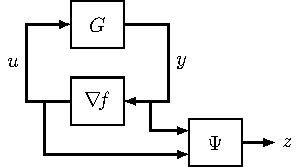
\includegraphics{text_figure} & 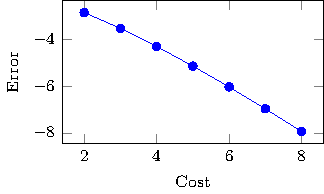
\includegraphics{test_plot}
	\end{tabular}
	\caption{Figure captions should be long and descriptive because people actually read them, unlike the rest of the text. (Left) A block diagram make using Tikz. (Right) A plot made using Pgfplots. Note that the figures are not scaled, so the text size in the figures is consistent with the rest of the document. The source files for the figures are in the \texttt{graphics/} folder.}
  \label{fig:sample}
\end{figure}

\paragraph{Tables}

The \verb|booktabs| package, which includes commands such as \verb|\toprule|, \verb|\midrule|, and \verb|\bottomrule|, can be used to make nice tables. In general, never use vertical lines to separate columns. For more style tips on how to make nice tables, see\footnote{\url{https://people.inf.ethz.ch/markusp/teaching/guides/guide-tables.pdf}}. Here is an example of a nice table\footnote{\url{https://lazyscientist.wordpress.com/2021/07/23/make-better-tables-in-latex-using-booktabs/}}.

\begin{table}[htbp]
	\centering
	\caption{Gravimetric analysis of silver halides in a 1.27-mL sample of sea water.}
	  \begin{tabular}{lSSSSS}
		  \toprule
		  \multicolumn{1}{c}{} & \multicolumn{4}{c}{Test Tubes} & \multicolumn{1}{c}{} \\
		  \cmidrule(rl){2-5} 
			Qty of Sample                & {A}           & {B}           & {C}           & {D}    & {Avg}             \\
		  \cmidrule(r){1-1} \cmidrule(rl){2-5} \cmidrule(l){6-6}
			Mass (g)                     & 1.399         & 1.32          & 1.328         & 1.408  & 1.364           \\
			Density (g/mL)               & 1.10          & 1.04          & 1.05          & 1.109  & 1.07            \\
			Mass w/ Precipitate (g)      & 13.443        & 13.401        & 13.348        & {---}  & 13.397          \\
			Mass AgCl (\num{e-2} g)      & 9.0           & 9.2           & 8.7           & {---}  & 8.9             \\
			Moles AgCl (\num{e-4} mol)   & 6.28          & 6.42          & 6.08          & {---}  & 6.50            \\
		  \bottomrule
	  \end{tabular}
	\label{tab:grav4}
\end{table}


%%%%%%%%%%%%%%%%%%%%%%%%%%%%%%%%%%%%%%%%%%%%%%%%%%%%%%%%%%%%%%%%%%%%%%%%%%%%%%%
%% APPENDICES
%%%%%%%%%%%%%%%%%%%%%%%%%%%%%%%%%%%%%%%%%%%%%%%%%%%%%%%%%%%%%%%%%%%%%%%%%%%%%%%
\appendices
\chapter{Background}

Use appendices to provide background information that the reader may already know, but is useful in case they need a refresher. A thesis on control, for example, may have an appendix on the linear--quadratic regulator, or some linear algebra.

\backmatter


%%%%%%%%%%%%%%%%%%%%%%%%%%%%%%%%%%%%%%%%%%%%%%%%%%%%%%%%%%%%%%%%%%%%%%%%%%%%%%%
%% BIBLIOGRAPHY
%%%%%%%%%%%%%%%%%%%%%%%%%%%%%%%%%%%%%%%%%%%%%%%%%%%%%%%%%%%%%%%%%%%%%%%%%%%%%%%
\addcontentsline{toc}{chapter}{References}
\renewcommand\bibname{References}
\bibliography{references}

\end{document}